Nachdem wir in Versuch 255 das Röntgenspektrum genauer untersucht hatten, setzen wir uns in Versuch 256 mit der sogenannten Röntgenfluoreszens auseinander. Röntgenfluoreszens beschreibt die Abstrahlung einer sekundären Röntgenstrahlung, bei der Interaktion von Röntgenstrahlung mit Materie.


\subsection{Physikalische Grundlagen}

Trifft Röntgenstrahlung auf Atome von Materie, kann diese Elektronen aus den inneren Schalen der Atome herauslösen. Rücken daraufhin Elektronen von den äußeren Schalen in die dadurch entstandenen Fehlstellen nach, so wird die dabei frei werdende Energie in Form einer sekundären Röntgenstrahlung abgestrahlt. Für die frei werdende Energie bei einem Elektronenübergang von der Schale $n_2$ zur Schale $n_1$ gilt, angenähert aus dem Bohr'schen Atommodell,
\begin{align}
  \Delta E = E_{2} - E_{1} = ch R_{\infty} \qty(\frac{(Z- \sigma_{n1})^2}{n_1^2} - \frac{(Z- \sigma_{n2})^2}{n_2^2}).
\end{align}
In diese Rechnung gehen neben der Lichtgeschwindigkeit $h$, dem Planck'schen Wirkungsquantum $h$ und der Rydberg-Konstante $R_{\infty}$ auch die Kernladungszahl $Z$ und die Abschirmkonstanten $\sigma_i$ ein, welche beide Materialabhängig sind. Daher ist die Röntgenfluoreszens charakteristisch für die bestrahlte Probe. Mit einer mittleren Abschirmkonstante $\sigma_{12}$, welche die $\sigma_{i}$ ersetzt und der Rydberg-Energie $E_{R} = ch R_{\infty}\, (\approx 13.6\si{\electronvolt})$ können wir die obige Gleichung umschreiben zu
\begin{align}
  \Delta E = E_2 - E_1 = E_{R} (Z - \sigma_{12})^2 \qty(\frac{1}{n_1^2} - \frac{1}{n_2^2}).
\end{align}

Betrachten wir speziell die $K_{\alpha}$-Strahlung der Übergänge $n_{2} = 2\to n_{1} = 1$, lässt sich die Abschirmkonstante für nicht zu schwere Kerne mit einer Ladungszahl bis etwa $Z \approx 30$ mit $\sigma_{12} \approx 1$ annähern. Damit können wir die Gleichung weiter vereinfachen zu
\begin{align}
  \sqrt{\frac{E}{E_R}} = (Z - 1) \sqrt{\frac{3}{4}}.
\end{align}

\subsubsection*{Röntgenenergiedetektor}

Im Versuch werden wir einen Halbleiterdetektor verwenden, um die Energie der Fluoreszenzstrahlung zu messen. Ein solcher Detektor ist aufgebaut wie eine in Sperrrichtung betriebene Diode, zu sehen in \abbref{fig:pn_halbleiter}. 
Hierbei werden ein n-Halbleiter, also ein Halbleiter mit einer erhöhten Anzahl an beweglichen negativen Ladungsträgern und ein p-Halbleiter mit einer erhöhten Anzahl an Fehlstellen in Kontakt gebracht. Aufgrund verschiedener Ladungsträgerdichten in den beiden Halbleitern kommt es an der Kontaktstelle zur Diffusion. Hierbei können Elektronen vom n-Halbleiter in den p-Halbleiter wandern und dort eine Fehlstelle besetzen. Es bildet sich die sogenannte Verarmungszone, in welcher keine freien Ladungsträger vorhanden sind. Durch die Ladungsträgerverschiebung baut sich ein elektrisches Feld auf, welches der Diffusion entgegenwirkt. Somit kann die Verarmungszone nicht beliebig groß werden. Durch eine von außen anliegende Spannung, welche umgekehrt zur Dotierung des Halbleiters gepolt ist, werden die freien Ladungsträger zusätzlich nach außen abgesaugt, wodurch sich die Verarmungszone weiter vergrößert. 

\begin{figure}[H]
  \centering
  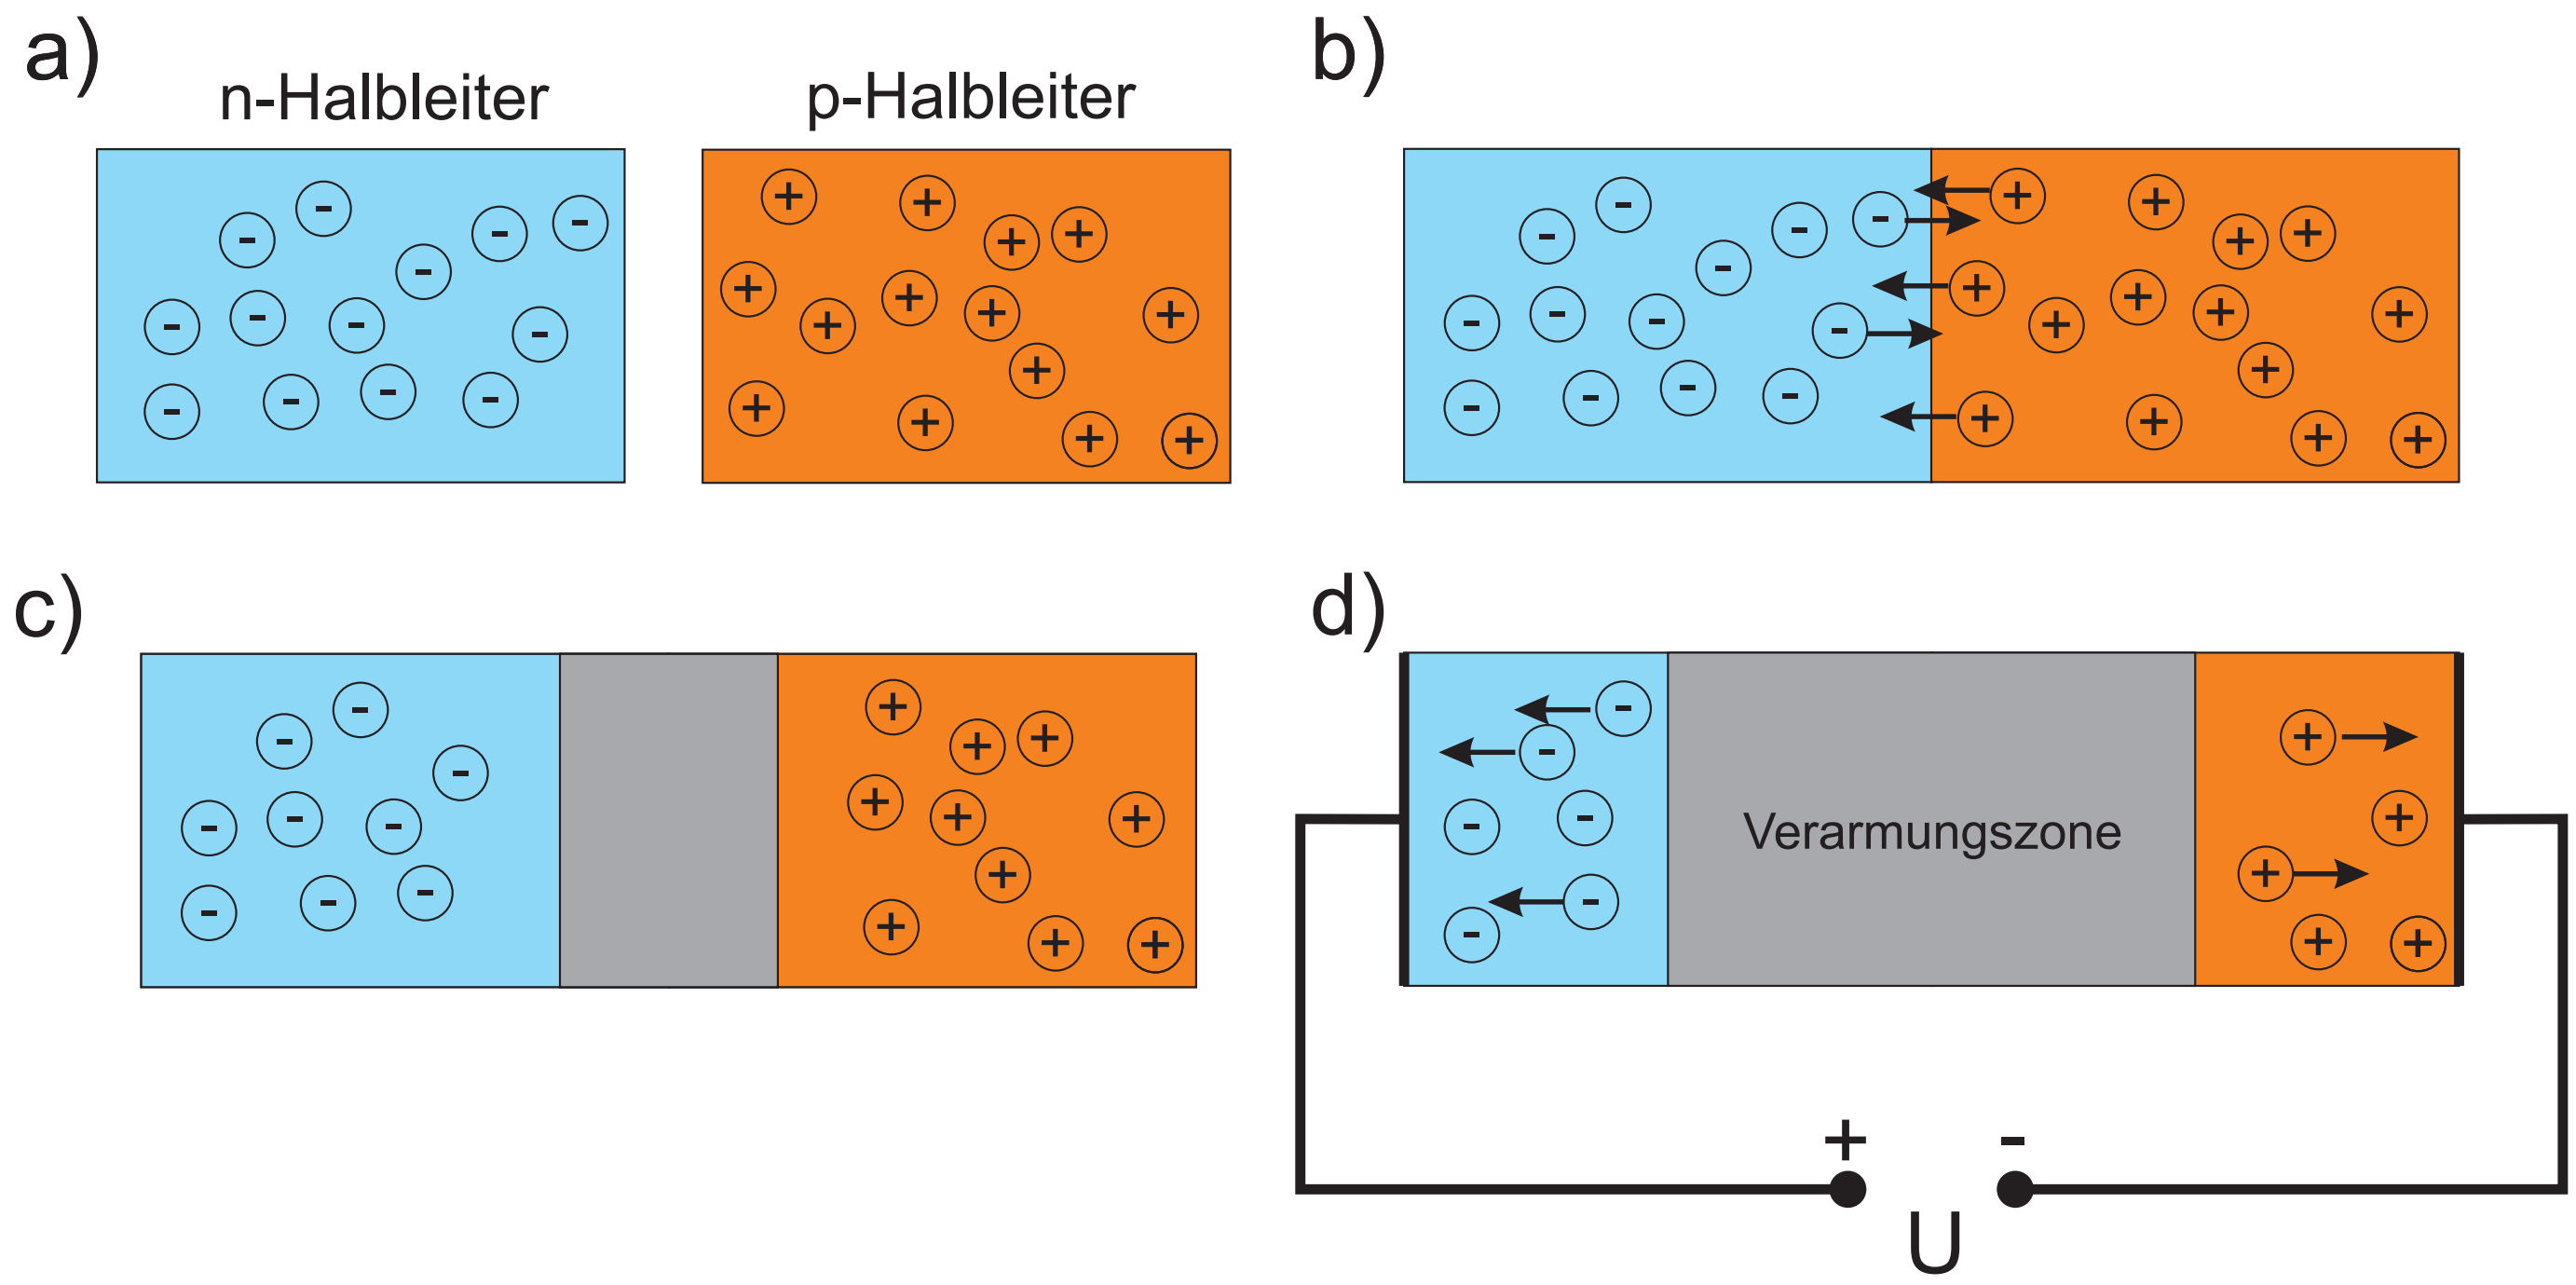
\includegraphics[width=.75\textwidth]{files/pn_halbleiter.png}
  \caption{Entstehung der Verarmungszone in einem pn-Halbleiter.}
  \label{fig:pn_halbleiter}
\end{figure}


Wenn ein Röntgenphoton auf die Verarmungszone trifft, wird dieses aufgrund des Photoeffekts absorbiert, wobei ein Photoelektron ausgesendet wird. Durch Stöße mit den Atomen der Halbleiter in der Verarmungszone werden Elektron-Loch-Paare zeugt, welche durch die anliegende Spannung abgesaugt werden. Dabei ist die Zahl der freigesetzten Ladungen proportional zur Energie des eingefallenen Röntgenphotons. Die ausgehenden Ladungsimpulse werden durch einen Integrator verstärkt und gemessen. Mit einem Vielkanalanalysator werden die verschiedenen Impulshöhen in Kanäle unterteilt und entsprechend der Häufigkeit, in der sie auftreten, in ein Histogramm zur Auswertung kategorisiert.

\begin{figure}[H]
  \centering
  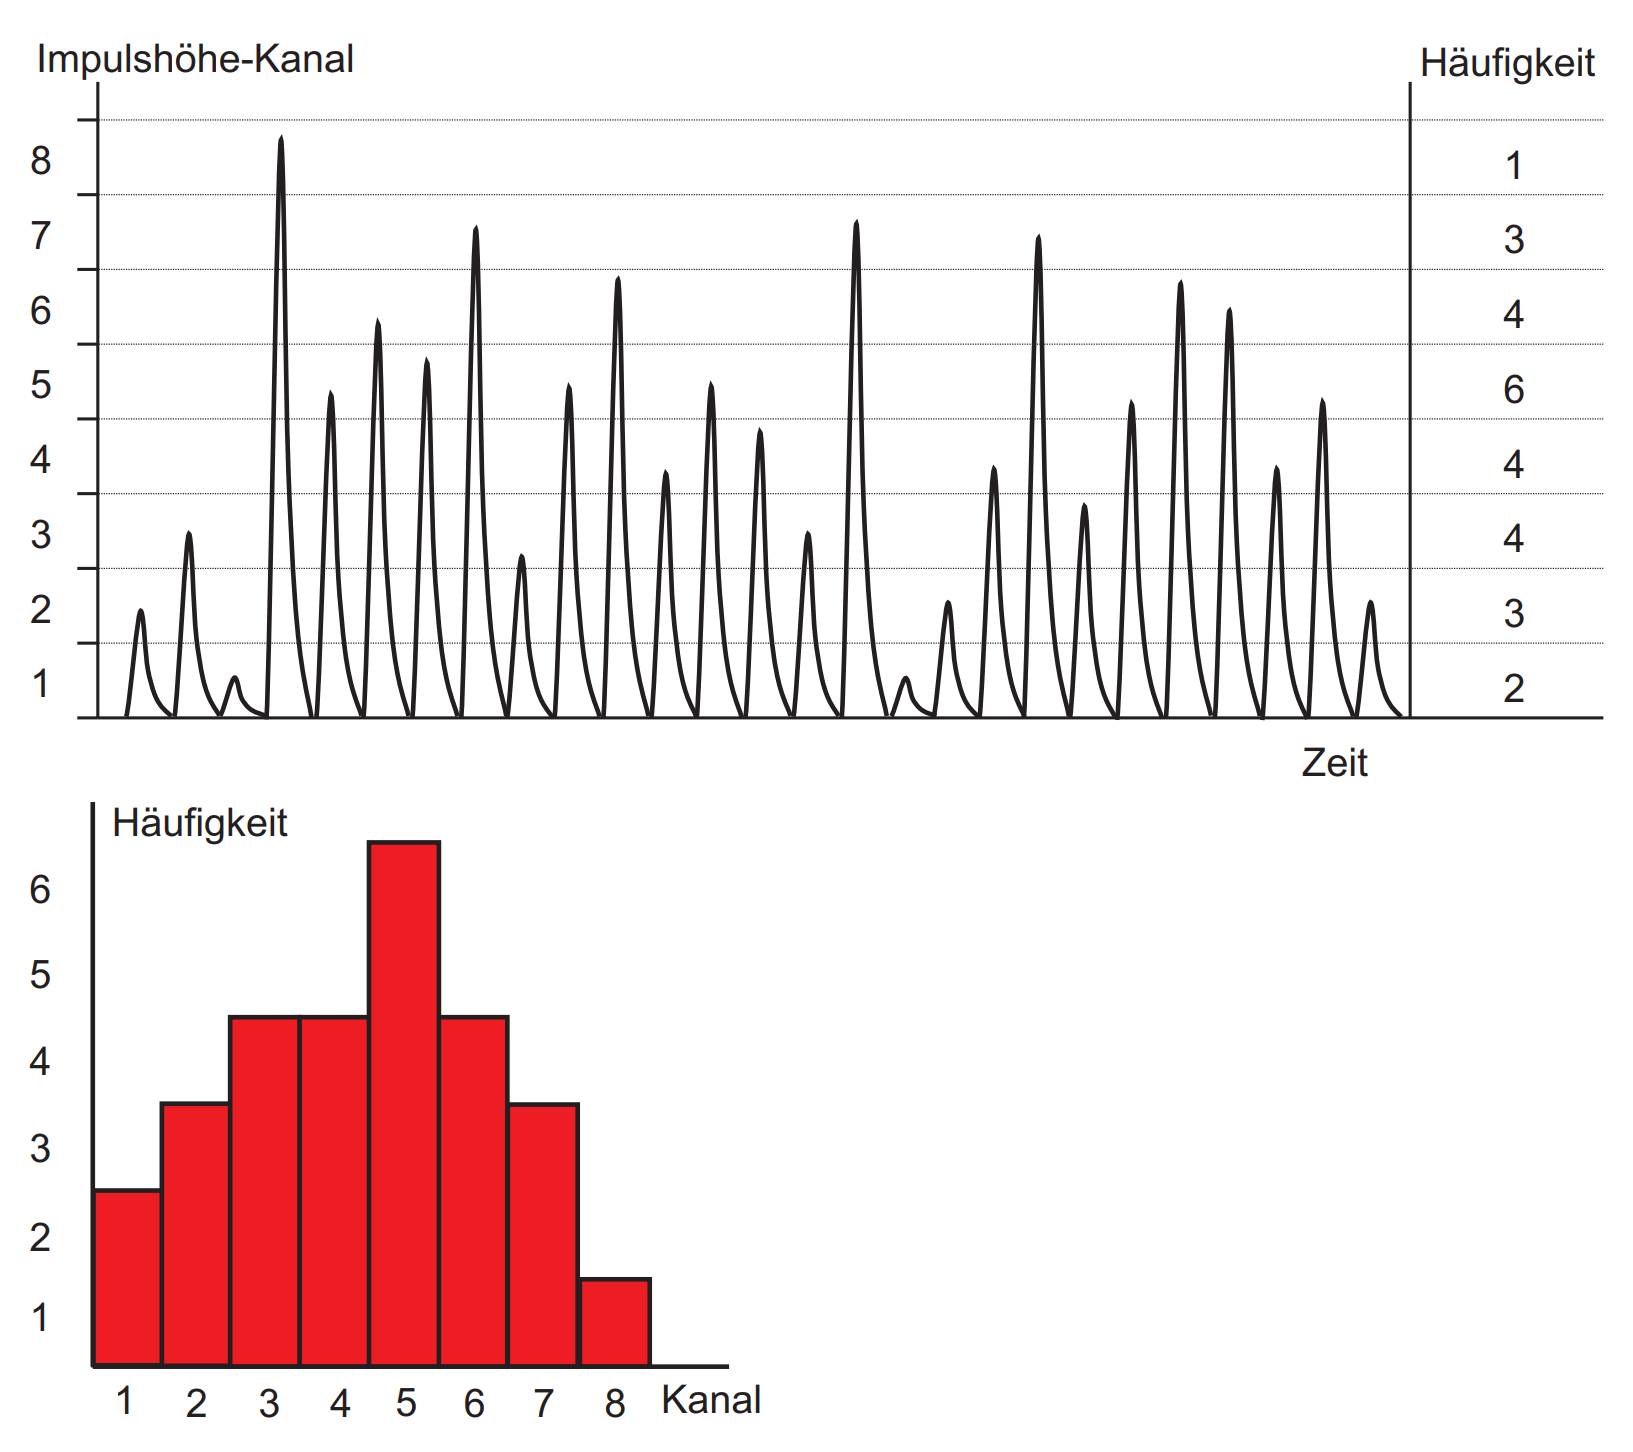
\includegraphics[width=.9\textwidth]{files/vielkanalanalysator.png}
  \caption{Funktionsprinzip des Vielkanalanalysators.}
  \label{fig:vielkanalanalysator}
\end{figure}

Entsprechend dem Energiespektrum eines bekannten Elements, in diesem Versuch sind das Eisen und Molybdän, kann die Umrechnung von der Kanalnummer zur entsprechenden Energie kalibriert werden.

\subsection{Versuchsdurchführung}

\textbf{Aufzeichnung der Impulse.} Im Röntgengerät ist der Targethalter in einem Winkel von $45\si{\degree}$ zur Strahlebene angebracht. Auf diesem positionieren wir nacheinander die verschiedenen Probenplättchen. Die Röntgenröhre wird mit einer Spannung von $35\si{\kilo\volt}$ und einem Strom von $1\si{\milli\ampere}$ betrieben. Wir zeichnen die Impulse über 512 Kanäle über eine Messzeit von $180\si{\second}$ pro Probe auf. Die Proben umfassen acht verschiedene reine Metalle und fünf verschiedene Legierungen.

\textbf{Energiekalibrierung.} Wir bestimmen zunächst die in der Analysesoftware im gemessenen Eisen- und Molybdänspektrum jeweils den Impulskanal des $K_{\alpha}$-Peaks. Wir kalibrieren die Energieskala, indem wir dann die bestimmten Impulskanäle mit den entsprechenden bekannten Energiewerten der $K_{\alpha}$-Strahlung der beiden jeweiligen Elemente assoziieren.

\textbf{Bestimmung der Lage der $K_{\alpha}$- und $K_{\beta}$-Peaks.} Anhand der nun kalibrierten Skala ermitteln wir Peakschwerpunkt ($\mu$) und Peakbreite ($\sigma$) der $K_{\alpha}$- und $K_{\beta}$-Peaks für alle aufgezeichneten Spektren der reinen Metalle.

\textbf{Untersuchung der Legierungen.} Anhand eines in der Analysesoftware integrierten Periodensystems, lassen sich die jeweiligen Energien in den aufgezeichneten Spektren ein- und ausblenden. Über die Zuordnung der dieser Energien zu den Peaks in den aufgezeichneten Spektren analysieren wir die Zusammensetzung der Legierungen.